\begin{frame}{Constitutional AI and RLAIF}
  \begin{center}
    \Large
    Constitutional AI and RLAIF
  \end{center}
\end{frame}

\begin{frame}[t]{Constitutional AI: Principles as Supervision}
  \begin{itemize}\itemsep0em
    \item[\textcolor{red}{$\blacktriangleright$}] \textbf{The problem with harmlessness data:} someone has to read the harmful output to label it. That does not scale, and it never says \emph{why} something was rejected: the rule lives in the labelers' heads.
    \item[\textcolor{red}{$\blacktriangleright$}] \textbf{Constitutional AI} (Bai et al., 2022) replaces those labels with a written list of principles, and gets the model to apply them to itself, in two stages:
      \begin{itemize}
        \item \textbf{SL-CAI (supervised).} Prompt a helpful-only model with red-team requests. Ask it to \emph{critique} its own response against a randomly sampled principle, then \emph{revise} it, and repeat. Fine-tune a pre-trained model on the revisions.
        \item \textbf{RL-CAI (reinforcement).} Sample response pairs from the SL-CAI model, ask a feedback model which one the sampled principle prefers, and train a preference model on those labels: AI-written for harmlessness, still human for helpfulness. Then run RLHF against it.
      \end{itemize}
    \item[\textcolor{red}{$\blacktriangleright$}] The RL stage used \textbf{16 principles}, one sampled at random per comparison, so no single wording dominates the preference model.
    \item[\textcolor{red}{$\blacktriangleright$}] The goal was a \emph{harmless but non-evasive} assistant: one that engages with a harmful request and explains its objection instead of refusing flatly.
  \end{itemize}
\end{frame}

\begin{frame}{Constitutional AI: The Two Stages}
  \begin{figure}
    \centering
    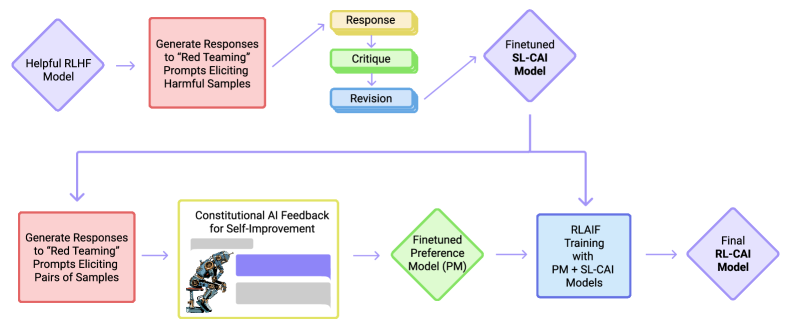
\includegraphics[width=0.84\paperwidth,height=0.50\paperheight,keepaspectratio]{images/llm-rlhf/constitutional_ai_two_stages.png}
    \caption*{\scriptsize Bai et al., ``Constitutional AI: Harmlessness from AI Feedback,'' \href{https://arxiv.org/abs/2212.08073v1}{arXiv:2212.08073v1}, Figure~1.}
  \end{figure}
\end{frame}

\begin{frame}[t,allowframebreaks]{RLAIF: Replacing the Human Labeler}
  \begin{itemize}\itemsep0.15em
    \item[\textcolor{red}{$\blacktriangleright$}] \textbf{Key idea:} Everything in the RLHF pipeline stays the same except who produces the preference labels. An off-the-shelf LLM reads the prompt and two candidates and picks one (Lee et al., 2024).
    \item[\textcolor{red}{$\blacktriangleright$}] The labeling prompt has four parts: a preamble stating the task, optional few-shot exemplars, the pair to annotate, and an ending such as ``\texttt{Preferred Response=}''. Asking the labeler for its reasoning first (chain of thought) generally improves agreement with humans.
    \item[\textcolor{red}{$\blacktriangleright$}] \textbf{LLM labelers have position bias:} which candidate is shown first shifts the answer. The fix is mechanical: label each pair twice with the order reversed, and average the two preference distributions.
    \item[\textcolor{red}{$\blacktriangleright$}] \textbf{d-RLAIF} goes one step further and deletes the reward model: score each rollout with the off-the-shelf LLM directly during RL. This avoids a reward model that goes stale as the policy moves away from the data it was fit on.
    \item[\textcolor{red}{$\blacktriangleright$}] \textbf{The economics:} human preference labels cost time and money per example; AI labels cost inference. The bottleneck moves from annotation throughput to having a labeler at least as capable as the model being aligned.
  \end{itemize}
\end{frame}

\begin{frame}{RLAIF Against RLHF}
  \begin{figure}
    \centering
    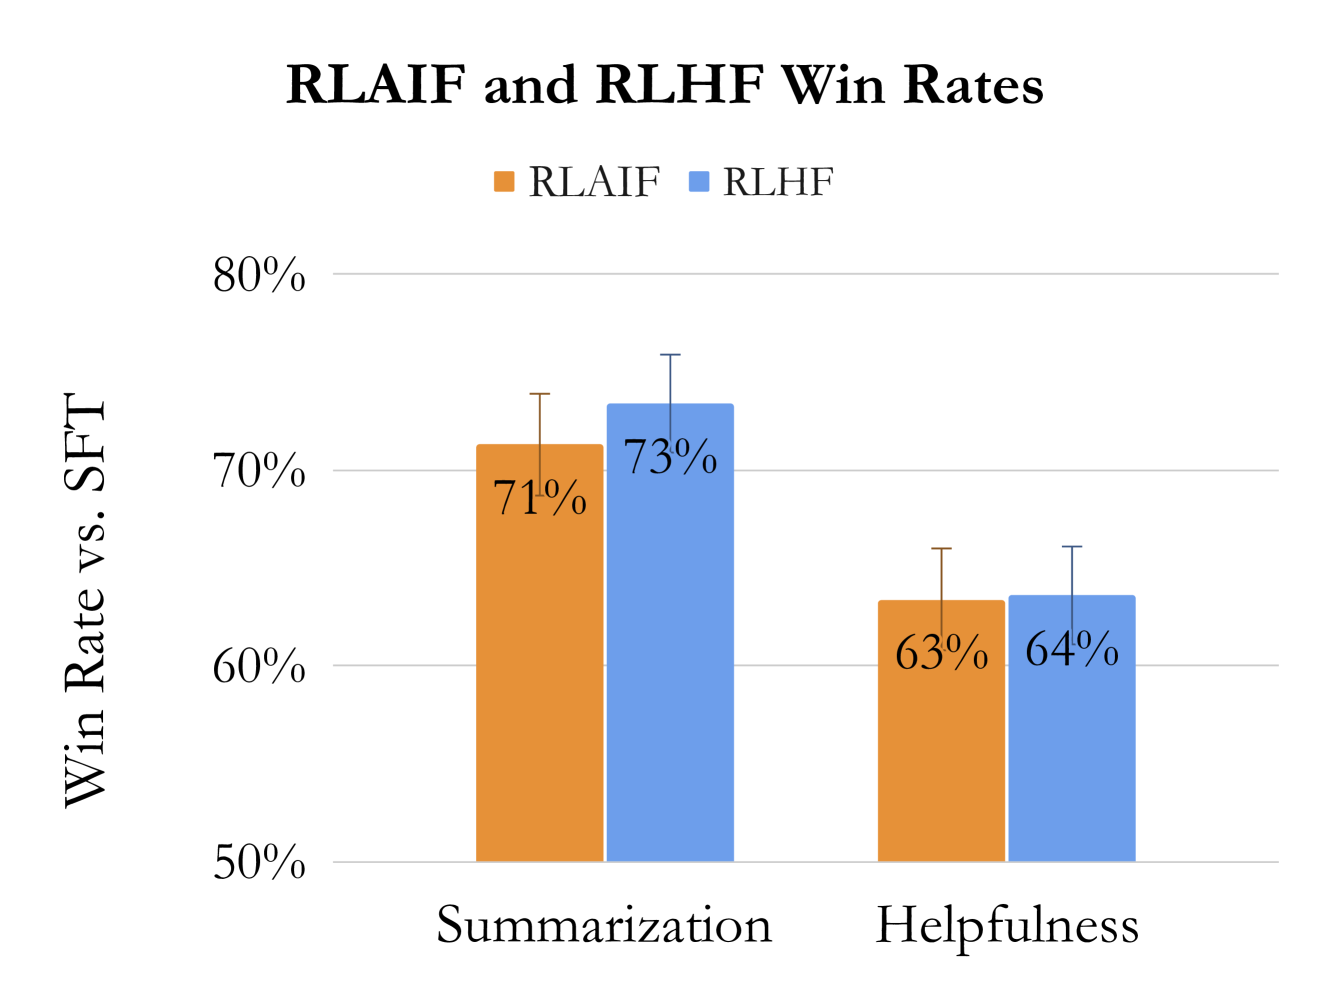
\includegraphics[width=0.44\paperwidth,height=0.56\paperheight,keepaspectratio]{images/llm-rlhf/rlaif_vs_rlhf_win_rates.png}
    \caption*{\scriptsize Lee et al., ``RLAIF vs.\ RLHF: Scaling Reinforcement Learning from Human Feedback with AI Feedback,'' \href{https://arxiv.org/abs/2309.00267v3}{arXiv:2309.00267v3}, Figure~1, left panel. Human-judged win rates against the SFT baseline.}
  \end{figure}
\end{frame}

\begin{frame}[t,allowframebreaks]{What AI Feedback Does and Does Not Buy}
  \begin{itemize}\itemsep0.35em
    \item[\textcolor{red}{$\blacktriangleright$}] \textbf{The headline result is parity.} Against an SFT baseline, human raters preferred RLAIF 71\% of the time on summarisation and RLHF 73\%; on helpful dialogue, 63\% and 64\%. Head to head the two are statistically indistinguishable: 50\% on summarisation, 52\% on dialogue.
    \item[\textcolor{red}{$\blacktriangleright$}] \textbf{On harmlessness the AI labeler was better:} 88\% harmless, against 76\% for RLHF and 64\% for the SFT baseline. This is the setting where the written principle is easiest to state and hardest for a tired human to apply consistently.
    \item[\textcolor{red}{$\blacktriangleright$}] \textbf{It works with a same-size labeler.} On summarisation, an RLAIF run whose labeler was the same size as the policy still beat the SFT baseline 68\% of the time, and d-RLAIF was preferred over that run 60/40. The gain is therefore not purely distillation from a larger model.
    \item[\textcolor{red}{$\blacktriangleright$}] \textbf{The values come from the labeler.} You are copying a preference distribution that some other alignment process produced. Its blind spots become yours, silently, and no amount of scale surfaces them, which is why \emph{evaluating} alignment is a separate discipline from producing it.
    \item[\textcolor{red}{$\blacktriangleright$}] \textbf{Looking ahead:} the same machinery now drives reasoning-model post-training, where the ``labeler'' is a verifier rather than a preference model. That story, and the RL algorithms built for it, belongs to a later session.
  \end{itemize}
\end{frame}
